\documentclass[11pt]{article}
\usepackage[ruled,]{algorithm2e}
\usepackage{naaclhlt2015}
\usepackage{times}
\usepackage{mathtools}
\usepackage{url}
\usepackage{latexsym}
\usepackage{amsfonts}
\usepackage{enumitem}
\usepackage{amsmath}
\usepackage{graphicx}
\usepackage{tabularx}
\usepackage{bm}
\usepackage{changepage}
%\usepackage{booktabs}
\usepackage{placeins}
\usepackage[normalem]{ulem}
\usepackage[table]{xcolor}
\usepackage{color, colortbl}
\newcommand{\cwindow}{1, 2, 4, 6, 8, 10, 12, 14, 15}
\newcommand{\cwinlen}{9}
\newcommand{\ctotalview}{16}
\newcommand{\xline}[0]{\noindent\underline{\makebox[0.1cm][l]{}}}
\newcommand{\specialcell}[2][c]{\begin{tabular}[#1]{@{}c@{}}#2\end{tabular}}
\newcommand{\mb}[1]{\textbf{#1}}
\newcommand{\ma}[1]{#1^\dagger}
\newcommand{\mi}[1]{\textbf{#1}}

\newcommand{\minimize}[3]{
\begin{aligned}
& \underset{#1}{\textrm{minimize:}}
& & #2 \\
& \textrm{subject to:}
& &  #3
\end{aligned}
}

%% Pretty fragile code to enable boldness and inheritance of separator.
\let\oldmc\multicolumn
\makeatletter
\newcolumntype{B}[3]{>{\boldmath\DC@{#1}{#2}{#3}}c<{\DC@end}}
\newcommand{\mcinherit}{\renewcommand{\multicolumn}[3]{\oldmc{##1}{##2}{\ifodd\rownum \@oddrowcolor\else\@evenrowcolor\fi ##3}}}
\makeatother
\newcommand{\m}[1]{\multicolumn{1}{c}{#1}}
\newcommand{\mm}[1]{\multicolumn{1}{c|}{#1}}
\newcommand{\mmm}[1]{\multicolumn{1}{c||}{#1}}
%\newcommand{\y}[1]{#1^*}
\newcommand{\y}[1]{\multicolumn{1}{B{.}{.}{-1}}{#1}}
\newcommand{\my}[1]{\multicolumn{1}{B{.}{.}{-1}}{#1}}
\newcommand{\myy}[1]{\multicolumn{1}{B{.}{.}{-1}|}{#1}}
\newcommand{\myyy}[1]{\multicolumn{1}{B{.}{.}{-1}||}{#1}}
\usepackage{array}
\usepackage{enumitem}
\usepackage{dcolumn}
\newcolumntype{H}{>{\setbox0=\hbox\bgroup}c<{\egroup}@{}}
\newcolumntype{d}[1]{D{.}{.}{#1}}
\newcolumntype{S}{l}
\newcolumntype{N}{>{\columncolor{green}}c}
\makeatletter
\newcommand{\R}{\mathbb{R}}
\newcommand{\remove}[1]{}
\newcommand{\removet}[1]{#1}
\newcommand*{\@rowstyle}{}
\newcommand*{\rowstyle}[1]{% sets the style of the next row
  \gdef\@rowstyle{#1}%
  \@rowstyle\ignorespaces%
}

\newcolumntype{=}{% resets the row style
  >{\gdef\@rowstyle{}}%
}

\newcolumntype{+}{% adds the current row style to the next column
  >{\@rowstyle}%
}

\newcommand{\raman}[1]{ (\textcolor{red}{Raman: #1})}

\definecolor{lightgray}{gray}{0.96}
\definecolor{darkgray}{gray}{0.7}
\definecolor{darkergray}{gray}{0.0}
%\setlength\titlebox{5cm}

% You can expand the titlebox if you need extra space
% to show all the authors. Please do not make the titlebox
% smaller than 5cm (the original size); we will check this
% in the camera-ready version and ask you to change it back.

\title{Multiview LSA: Representation Learning via Generalized CCA}

\author{Pushpendre Rastogi$^1$ \and Benjamin Van Durme$^{1,2}$ \and Raman Arora$^{1}$\\
  $^1$Center for Language and Speech Processing\\
    $^2$Human Language Technology Center of Excellence\\
    Johns Hopkins University}

\date{}

\begin{document}
\maketitle
\begin{abstract}
  \emph{Multiview LSA (MVLSA)} is a generalization of Latent Semantic
  Analysis (LSA) that supports the
  fusion of arbitrary views of data and relies on Generalized Canonical Correlation
  Analysis (GCCA). We present an algorithm
  for fast approximate computation of GCCA, which when coupled with methods
  for handling missing values, is general enough to approximate
  some recent algorithms for inducing vector representations of
  words. Experiments across a comprehensive
  collection of test-sets show our approach to be competitive with the
  state of the art.
\end{abstract}

\section{Introduction}
\newcite{winograd1972understanding} wrote that: \emph{``Two sentences
  are paraphrases if they produce the same representation in the
  internal formalism for meaning''}.  This intuition is made soft in
vector-space models \cite{turney2010frequency}, where we say that
expressions in language are paraphrases if
their representations are \emph{close} under some distance measure.

One of the earliest linguistic vector space models was Latent
Semantic Analysis (LSA). LSA has been successfully used
for Information Retrieval but it is limited in its
reliance on a single matrix, or \emph{view}, of term co-occurrences.
Here we address the single-view limitation of LSA by demonstrating
that the framework of Generalized Canonical Correlation Analysis
(GCCA) can be used to perform Multiview LSA (MVLSA). This
approach allows for the use of an arbitrary number of views in the
induction process, including embeddings induced using other
algorithms. We also present a fast approximate method for performing
GCCA and approximately recover the objective of
\cite{pennington2014glove} while accounting for missing values.

Our experiments show that MVLSA is competitive with state of the art
approached for inducing vector representations of words and phrases.
As a methodological aside, we discuss the \mbox{(in-)significance} of
conclusions being drawn from comparisons done on small sized datasets.

\section{Motivation}
LSA is an application of Principal Component Analysis (PCA) to a
term-document cooccurrence matrix.  The principal directions found by
PCA form the basis of the vector-space in which to represent the input
terms~\cite{landauer1997solution}. A drawback of PCA is that it can
leverage only a single source of data and it is sensitive to scaling.

An arguably better approach to representation learning is Canonical
Correlation Analysis (CCA) that induces representations that are
maximally \emph{correlated} across two views, allowing the utilization
of two distinct sources of data. While an improvement over PCA, being
limited to only two views is unfortunate in light of the fact that
many sources of data (perspectives) are frequently available in
practice.  In such cases it is natural to extend CCA's original
objective of maximizing correlation between two views by maximizing
some measure of the matrix $\Phi$ that contains all the pairwise
correlations between linear projections of the \emph{covariates}. This
is how Generalized Canonical Correlation Analysis (GCCA) was first
derived by~\newcite{horst1961generalized}. Recently these intuitive
ideas about benefits of leveraging multiple sources of data have
received strong theoretical backing due to the work by
\newcite{sridharan2008information} who showed that learning with
multiple views is beneficial since it reduces the complexity of the
learning problem by restricting the search space.  Recent work by
\newcite{anandkumar2014tensor} showed that at least three views are
necessary for recovering hidden variable models.

Note that there exist different variants of GCCA depending on the
measure of $\Phi$ that we choose to
maximize. \newcite{kettenring1971canonical} enumerated a variety of
possible measures, such as the spectral-norm of $\Phi$. Kettenring
noted that maximizing this spectral-norm is equivalent to finding
linear projections of the \emph{covariates} that are most amenable to
rank-one PCA, or that can be best explained by a single term factor
model. This variant was named \emph{MAX-VAR GCCA} and was shown to be
equivalent to a proposal by \newcite{carroll1968generalization}, which
searched for an auxiliary orthogonal representation $G$ that was
maximally correlated to the linear projections of the
covariates.  Carroll's objective targets the intuition
that representations leveraging multiple views should correlate with
all provided views as much as possible.

\section{Proposed Method: MVLSA}
\label{sec:gcca}
Let $X_j \in \mathbb{R}^{N\times d_j} \;
\forall j \in [1,\ldots,J]$ be the mean centered matrix containing
data from view $j$ such that row $i$ of $X_j$ contains the information for
word $w_i$. Let the number of words in the vocabulary be $N$
and number of contexts (columns in $X_j$) be $d_j$. %% Note that $N$
%% remains the same and $d_j$ varies across views.
Following standard
notation \cite{hastie2009elements} we call $X_j^\top X_j$ the scatter
matrix and $X_j (X_j^\top X_j)^{-1}X_j^\top$ the projection matrix.

The objective of \emph{MAX-VAR GCCA} can be written as the following optimization problem:
 Find $G \in \mathbb{R}^{N\times r}$ and $U_j \in
\mathbb{R}^{d_j \times r}$ that solve:
\begin{equation}
  \label{eq:gcca}
\begin{split}
  \operatorname*{\arg\,\min}_{G,U_j} & \sum_{j=1}^J \begin{Vmatrix} G - X_jU_j \end{Vmatrix}^2_F \\
  \text{subject to } & G^\top G = I.
\end{split}
\end{equation}
% The matrix $G$ that satisfies expression~\ref{eq:gcca} would also be our vector representation of the vocabulary.
The matrix $G$ that solves problem~(\ref{eq:gcca}) is our vector representation of the vocabulary. Finding $G$ reduces to spectral decomposition of sum of projection matrices of different views: Define
\begin{align}
P_j =& X_j(X_j^\top X_j)^{-1}X_j^\top, \label{eq:pp}\\
M =& \sum_{j=1}^J P_j. \label{eq:mm}
\end{align}
Then, for some positive diagonal matrix $\Lambda$, $G$ and $U_j$ satisfy:
\begin{align}
M G =& G \Lambda,\\
U_j =& \left(X_j^\top X_j\right)^{-1} X_j^\top G.
\end{align}

%% The above expressions tell us that our word representations are the
%% eigenvectors of the sum of $J$ projection matrices. Also note that the
%% dimensions of $G$ are orthogonal to each other. %% Orthogonality in
%% representations is a nice property that we
%% will discuss later.

Computationally storing $P_j \in \mathbb{R}^{N \times N}$ is
problematic owing to memory constraints.  Further, the scatter
matrices may be non-singular leading to an ill-posed procedure.
% Let us now describe a method to overcome these problems.
We now describe a novel scalable GCCA with $\ell_2$-regularization to address these issues.

\noindent\textbf{Approximate Regularized GCCA}: GCCA can be regularized by adding $r_jI$ to
scatter matrix $X_j^\top X_j$ before doing the inversion where
$r_j$ is a small constant e.g. $10^{-8}$.
% Equations~\ref{eq:pp} and \ref{eq:mm} change to
Projection matrices in~(\ref{eq:pp}) and (\ref{eq:mm}) can then be written as
\begin{align}
  \widetilde{P}_{j} =& X_j(X_j^\top X_j+r_jI)^{-1}X_j^\top, \label{eq:6}\\
  M =& \sum_{j=1}^J \widetilde{P}_{j}. \label{eq:mmm}
\end{align}

% We can side step the computational difficulties by assuming that only the top $m$ singular values of $X_j$ are non-negligible. Parts of the following method were proposed to us by \cite{savostyanov}.
Next, to scale up GCCA to large datasets, we first form a rank-$m$ approximation of projection matrices~\cite{arora2012kernel} and then extend it to an eigendecomposition for $M$ following ideas by~\newcite{savostyanov}. Consider the rank-$m$ SVD of $X_j$:
$$X_j = A_{j} S_{j} B^\top_{j},$$
where $S_j \in \R^{m \times m}$ is the diagonal matrix with $m$-largest singular values of $X_j$ and $A_j \in \R^{N \times m}$ and $B_j \in \R^{m \times d_j}$ are the corresponding left and right singular vectors. Given this SVD, write the $j^{th}$ projection matrix as
\begin{eqnarray}
\widetilde{P}_j &=& A_j S_j^\top(r_j I + S_j S_J^\top)^{-1}S_j A_j^\top, \nonumber \\
&=& A_j T_j T_j^\top A_j^\top, \nonumber
\end{eqnarray}
where $T_j \in \mathbb{R}^{m \times m}$ is a diagonal matrix such that
$T_jT_j^\top = S_j^\top(r_j I + S_j S_J^\top)^{-1}S_j$. Finally, we note that the sum of projection matrices can be expressed as $M = \tilde{M} \tilde{M}^\top$
where $$\tilde{M} = \left[ A_1T_1 \ldots A_JT_J \right] \in \mathbb{R}^{N
  \times mJ}.$$
Therefore, eigenvectors of matrix $M$, i.e. the matrix $G$ that we are interested in finding, are the left singular vectors of $\tilde{M}$, i.e. $\tilde{M}=GSV^\top$. These left singular vectors can be computed by using Incremental PCA \cite{brand2002incremental} since $\tilde{M}$ may be too large to fit in memory.

\subsection{Computing SVD of mean centered $X_j$}
\label{ssec:svdmc}
Recall that we assumed $X_j$ to be mean centered matrices. Let $Z_j
\in \mathbb{R}^{N \times d_j}$ be sparse matrices containing
mean-uncentered cooccurrence counts. Let $f_j = n_j \circ t_j $ be the preprocessing
function that we apply to $Z_j$:
\begin{align}
  Y_j =& f_j (Z_j), \\
  X_j =& Y_j - 1 (1^\top Y_j).
\end{align}
In order to compute the SVD of mean centered matrices $X_j$ we first
compute the partial SVD of uncentered
matrix $Y_j$ and then update it (\newcite{brand2006fast} provides details).
We experimented with representations created from the
uncentered matrices $Y_j$ and found that they performed as well as
the mean centered versions but we would not mention them further since
it is computationally efficient to follow the principled approach. We
note, however, that even the method of mean-centering the SVD
produces an approximation.

\subsection{Handling missing rows across views}
\label{ssec:missing}
With real data it may happen that a term was not observed in a view at
all. A large number of
missing rows can corrupt the learnt representations since the rows
in the left singular matrix become zero.
\remove{The procedure described above
can not recover from this and the representation for those words may become a
one hot vector. }
To counter this problem we adopt a variant of the ``missing-data
passive'' algorithm from \newcite{van2006generalized} who modified the
GCCA objective to counter the problem of missing
rows.\footnote{A more recent effort, by \newcite{van2012generalized},
  describes newer iterative and non-iterative (Test-Equating Method)
  approaches for handling missing values. It is possible that using
  one of those methods could improve performance. \label{ftn:mis}}
The objective now becomes:
\begin{equation}
  \label{eq:gcca2}
\begin{split}
  \operatorname*{arg\,min}_{G,U_j} & \sum_{j=1}^J \begin{Vmatrix} K_j(G - X_jU_j) \end{Vmatrix}^2_F \\
  \text{subject to } & G^\top G = I,
\end{split}
\end{equation}
where $[K_j]_{ii} = 1$ if row $i$ of view $j$ is observed and zero otherwise. Essentially $K_j$ is a diagonal row-selection matrix which ensures
that we optimize our representations only on the observed rows. Note that
$X_j = K_jX_j$ since the rows that $K_j$ removed were already
zero. Let, $K =
\sum_j K_j$ then the optima
of the objective can be computed by modifying equation~(\ref{eq:mmm}) as:
\begin{align}
  M =& K^{-\frac{1}{2}}(\sum_{j=1}^J P_j)K^{-\frac{1}{2}}.
\end{align}
Again, if we regularize and approximate the GCCA solution we get
$G$ as the left singular vectors of $K^{-\frac{1}{2}}\tilde{M}$. We mean center the matrices using only the observed rows.

Also note that other heuristic weighting schemes could be used
here. For example if we modify our objective as follows then we would
approximately recover the objective of \newcite{pennington2014glove}:

\begin{eqnarray}
  \label{eq:gcca3}
\minimize{G,U_j}{\sum_{j=1}^J \begin{Vmatrix} W_j K_j(G - X_jU_j) \end{Vmatrix}^2_F}{G^\top G = I }
\end{eqnarray}

where
\begin{eqnarray}
[W_j]_{ii} &=& \left(\frac{w_i}{w_{\max}}\right)^{\frac{3}{4}} \text{ if } w_i <
  w_{\max} \text{ else } 1, \nonumber \\
  \text{and } w_i &=&  \sum_k [X_j]_{ik}. \nonumber
\end{eqnarray}


\section{Data}
\label{sec:data}

\noindent\textbf{Training Data} We used the English portion of the
\textit{Polyglot} Wikipedia dataset released by
\newcite{al2013polyglot} to create 15 \emph{irredundant} views of
cooccurrence statistics where element $[z]_{ij}$ of view $Z_k$
represents that number of times word $w_j$ occurred $k$ words behind
$w_i$. We selected the top 500K words by occurrence to create our
vocabulary for the rest of the paper.

%% \remove{We lowercased all the words and discarded all
%% words which were longer than 5 characters and contained more than 3 non
%% alphabetical symbols. This was done to preserves years and smaller
%% numbers.}

We extracted cooccurrence statistics from a large bitext corpus that
was made by combining a number of parallel bilingual corpora as part
of the ParaPhrase DataBase (PPDB) project: Table~\ref{tab:dataperlang}
gives a summary, \newcite{ganitkevitch2013ppdb} provides further
details. Element $[z]_{ij}$ of the \textit{bitext} matrix represents
the number of times English word $w_i$ was automatically aligned to
the foreign word $w_j$.

We also used the dependency relations in the \textit{Annotated
  Gigaword Corpus}~\cite{annotatedGigaword12} to create 21
views\footnote{Dependency relations employed: nsubj, amod, advmod, rcmod, dobj, prep\xline{}of,
  prep\xline{}in, prep\xline{}to, prep\xline{}on, prep\xline{}for,
  prep\xline{}with, prep\xline{}from, prep\xline{}at, prep\xline{}by,
  prep\xline{}as, prep\xline{}between, xsubj, agent, conj\xline{}and,
  conj\xline{}but, pobj.}  where element $[z]_{ij}$ of view
$Z_d$ represents the number of times word $w_j$ occurred
as the governor of word $w_i$ under dependency relation $d$.

%% We selected these dependency relations since
%%   they seemed to be the particularly interesting which could capture
%%   different aspects of similarity.


We combined the knowledge of paraphrases present in FrameNet and PPDB
by using the dataset created by \newcite{rastogi2014augmenting} to
construct a \textit{FrameNet} view. Element $[z]_{ij}$ of the
\textit{FrameNet} view represents whether word $w_i$ was present in
frame $f_j$. Similarly we combined the knowledge of morphology present
in the \textit{CatVar} database released by \newcite{habash2003catvar}
and \textit{morpha} released by \newcite{minnen2001applied} along with \textit{morphy} that is a part of WordNet.
The morphological views and the frame semantic views were especially
sparse with densities of 0.0003\% and 0.03\%. While the approach
allows for an arbitrary number of distinct sources of semantic
information, such as going further to include cooccurrence in WordNet
synsets, we considered the described views to be representative, with
further improvements possible as future work.
%%Figure~\ref{fig:cartoon} summarizes our description.


\begin{figure}
  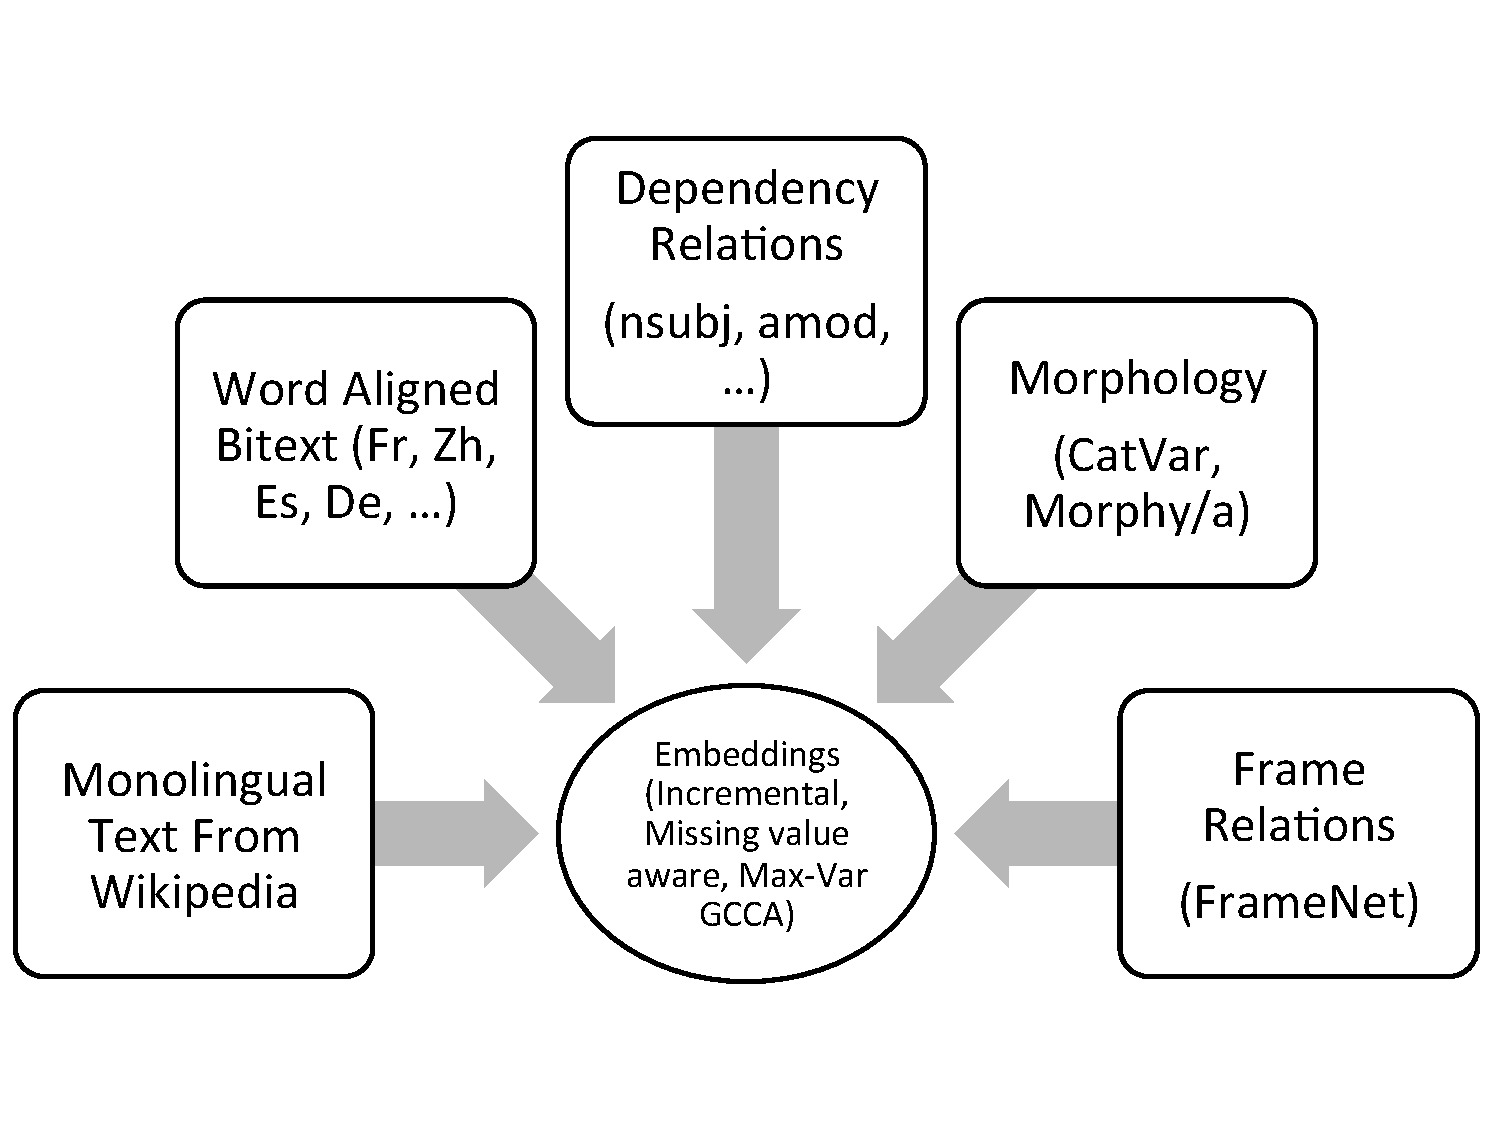
\includegraphics[trim=0 70 0 35,clip,width=\linewidth]{cartoonbw.pdf}
  \caption{An illustration of datasets used.}
  \label{fig:cartoon}
  \end{figure}


\begin{table}[htbp]
  \centering
  \rowcolors{1}{}{lightgray}
  \begin{tabular}{lrr}
    Language & Sentences & English Tokens \\
    \hline
    Bitext-Arabic   & 8.8M   & 190M  \\
    Bitext-Czech    & 7.3M   & 17M   \\
    Bitext-German   & 1.8M   & 44M   \\
    Bitext-Spanish  & 11.1M  & 241M  \\
    Bitext-French   & 30.9M  & 671M  \\
    Bitext-Chinese  & 10.3M  & 215M  \\
    Monotext-En-Wiki& 75M    & 1700M
  \end{tabular}
  \caption{Portion of data used to create GCCA representations (in millions).}
  \label{tab:dataperlang}
\end{table}

\noindent\textbf{Test Data} We evaluated the representations on the
word similarity datasets listed in Table~\ref{tab:testlist}. The first
10 datasets in Table~\ref{tab:testlist} were annotated with different
rubrics and rated on different scales. But broadly they all
contain human judgements about how similar two words are.
The ``AN-SYN'' and ``AN-SEM'' datasets contain 4-tuples of
analogous words and the task is to predict the missing word given the
first three. Both of these are  open vocabulary tasks while TOEFL is a closed
vocabulary task.
\begin{table*}[ht]
  \centering
  \rowcolors{1}{}{lightgray}
  \begin{tabular}{lr | ccc  | ccc | l}
    Acronym & Size  &
    $\sigma_{0.01}^{0.5}$ & $\sigma_{0.01}^{0.7}$ & $\sigma_{0.01}^{0.9}$ &
    $\sigma_{0.05}^{0.5}$ & $\sigma_{0.05}^{0.7}$ & $\sigma_{0.05}^{0.9}$ &
    Reference  \\
    \hline

    MEN    & 3000  & 4.2  & 3.2  & 1.8  & 3.0  & 2.3  & 1.3  & \cite{bruni2012distributional}  \\
    RW     & 2034  & 5.1  & 3.9  & 2.3  & 3.6  & 2.8  & 1.6  & \cite{Luong2013morpho}          \\
    SCWS   & 2003  & 5.1  & 4.0  & 2.3  & 3.6  & 2.8  & 1.6  & \cite{Huang2012Improving}       \\
    SIMLEX & 999   & 7.3  & 5.7  & 3.2  & 5.2  & 4.0  & 2.3  & \cite{hill2014simlex}           \\
    WS     & 353   & 12.3 & 9.5  & 5.5  & 8.7  & 6.7  & 3.9  & \cite{finkelstein2001placing}   \\
    MTURK  & 287   & 13.7 & 10.6 & 6.1  & 9.7  & 7.5  & 4.3  & \cite{Radinsky2011word}         \\
    WS-REL & 252   & 14.6 & 11.3 & 6.5  & 10.3 & 8.0  & 4.6  & \cite{agirre2009study}          \\
    WS-SEM & 203   & 16.2 & 12.6 & 7.3  & 11.5 & 8.9  & 5.1  & -Same-As-Above-                 \\
    RG     & 65    & 28.6 & 22.3 & 12.9 & 20.6 & 16.0 & 9.2  & \cite{Rubenstein1965Contextual} \\
    MC     & 30    & 41.7 & 32.7 & 19.0 & 30.6 & 23.9 & 13.8 & \cite{miller1991contextual}     \\ \hline
    AN-SYN  & 10675 & -    & -    & 0.95 & -    & -    & 0.68 & \cite{mikolov2013distributed}   \\
    AN-SEM  & 8869  & -    & -    & 1.03 & -    & -    & 0.74 & -Same-As-Above-                 \\
    TOEFL  & 80    & -    & -    & 8.13 & -    & -    & 6.63 & \cite{landauer1997solution}
  \end{tabular}
  \caption{List of test datasets used. The columns headed $\sigma_{p_0}^r$ contain
    \emph{MRDS}
    values. The rows for accuracy based test sets contain
    $\sigma_{p_0}$ which does not depend on $r$. See
    \S~\ref{ssec:mrds} for details.}
   \label{tab:testlist}
\end{table*}

\subsection{Significance of comparison} \label{ssec:mrds}
While surveying the literature we found that performance on word
similarity datasets is typically reported in terms of the Spearman
correlation between the gold ratings and the cosine distance between
normalized embeddings.  However researchers do not report measures of
significance of the difference between the Spearman Correlations even
for comparisons on small evaluation sets.\footnote{For example, the
  comparative difference by competing algorithms reported by
  \newcite{faruqui2014retrofitting} could not be significant for the
  Word Similarity test set released by
  \newcite{finkelstein2001placing}, even if we assumed a correlation
  between competing methods as high as 0.9, with a p value threshold of
  0.05.  Similar such comparisons on small datasets are
  performed by \newcite{hill2014not}.} This motivated our defining a
method for calculating the \emph{Minimum Required Difference for
  Significance (MRDS)}.

\noindent\textbf{Minimum Required Difference for Significance (MRDS)}:
Imagine two lists of ratings over the same items, produced
respectively by algorithms $A$ and $B$, and then a list of gold
ratings $T$. Let $r_{AT}$, $r_{BT}$ and $r_{AB}$ denote the Spearman
correlations between $A:T$, $B:T$ and $A:B$ respectively. Let
$\hat{r}_{AT}, \hat{r}_{BT}, \hat{r}_{AB}$ be their empirical
estimates and assume that $\hat{r}_{BT} > \hat{r}_{AT}$ without loss
of generality.

For word similarity datasets we define $\sigma_{p_0}^r$ as the MRDS,
such that it satisfies the following proposition: {\small $$ (r_{AB} <
  r) \land (|\hat{r}_{BT} - \hat{r}_{AT}|{<}\sigma_{p_0}^r) {\implies}
  \textit{pval} > p_0$$}. Here $\textit{pval}$ is the probability of
the test statistic under the null hypothesis that $r_{AT} = r_{BT}$
found using the Steiger's test \cite{steiger1980tests}. The above
constraint ensures that as long as the correlation between the
competing methods is less than $r$ and the difference between the
correlations of the scores of the competing methods to the gold
ratings is less than $\sigma_{p_0}^r$, then the pvalue of the null
hypothesis will be greater than $p_0$.  We can then ask what we
consider a reasonable upper bound on the agreement of ratings produced
by competing algorithms: for instance two algorithms correlating above
$0.9$ might not be considered meaningfully different.  That leaves us
with the second part of the predicate which ensures that as long as
the difference between the correlations of the competing algorithms to
the gold scores is less than $\sigma_{p_0}^r$ then the null hypothesis
is more likely than $p_0$.

We can find $\sigma_{p_0}^r$ as follows: Let $\textit{stest}$
denote Steiger's test predicate which satisfies the following:
$$\textit{stest-p}(\hat{r}_{AT}, \hat{r}_{BT}, r_{AB}, p_0, n)
{\implies} \textit{pval} < p_0$$ Once we define this predicate then we
can use it to set up an optimistic problem where our aim is to find
$\sigma_{p_0}^r$ by solving the following: {\small $$\sigma_{p_0}^r =
  \min\{\sigma | \forall\, 0 {<} r' {<} 1\, \textit{stest-p}(r',
  \min(r'+\sigma, 1), r, p_0, n) \} $$} Note that MRDS is a liberal
threshold and it only guarantees that differences in correlations
below that threshold can never be statistically significant (under the
given parameter settings). MRDS might optimistically consider some
differences as significant when they are not, but it is at least
useful in reducing some of the noise in the evaluations.  The values
of $\sigma_{p_0}^r$ are shown in Table~\ref{tab:testlist}.

For the accuracy based test-sets we found MRDS$=\sigma_{p_0}$ that satisfied
the following:
{\small $$ 0< (\hat{\theta}_{B} - \hat{\theta}_{A})<\sigma_{p_0}
  {\implies} \text{p}(\theta_{B} \le \theta_{A}) > p_0$$}
Specifically, we calculated the posterior probability
$\text{p}(\theta_{B} \le \theta_{A})$ with a flat prior of
$\beta(1,1)$ to solve the following:\footnote{This instead of using  McNemar's test
  \cite{mcnemar1947note} since the Bayesian approach is tractable and
  more direct. A calculation with $\beta(0.5, 0.5)$ as the prior
  changed $\sigma_{0.5}$ from 6.63 to 6.38 for the TOEFL dataset but
  did not affect MRDS for the AN-SEM and AN-SYN datasets.}
{\small $\sigma_{p_0}=\min\{\sigma |\forall\,
  0{<}\theta{<}\min(1{-}\sigma,0.9)\,$
  $\text{p}(\theta_{B}{\le} \theta_{A}| \hat{\theta}_A{=}\theta,
\hat{\theta}_B{=}\theta+\sigma, n) < p_0\}$}
Here $\theta_{A}$ and $\theta_{B}$ are probability of correctness of
algorithms $A$, $B$ and $\hat{\theta}_{A}$, $\hat{\theta}_{B}$ are
observed empirical accuracies.

Unfortunately there are no widely reported train-test splits of the
above datasets, leading to potential concerns of \emph{soft
  supervision} (hyper-parameter tuning) on these evaluations, both in
our own work and throughout the existing literature.  We report on the
resulting impact of various parameterizations, and our final results
are based on a single set of parameters used across all evaluation
sets.

%% Here we follow
%% this accepted practice, but on ongoing work are exploring evaluation
%% of these learned representations in downstream systems as


%% and we also evaluated the effects of hyper-parameter tuning
%% on the entire test set therefore our final comparison could have
%% favored us due to \emph{soft supervision}.
%% However the consistent performance of our
%% method across the test sets lends hope that the trends we report would
%% generalize.


\section{Experiments and Results}
\label{sec:exp}
We wanted to answer the following questions through our experiments:
(1) How do hyper-parameters affect performance? (2) What is the
contribution of the multiple sources of data to performance? (3) How
does the performance of MVLSA compare with other methods? For brevity
we show tuning runs only on the larger datasets. We also highlight the top
performing configurations in bold using the small threshold values in
column~$\sigma_{0.05}^{0.09}$ of Table~\ref{tab:testlist}.

\noindent\textbf{Effect of Hyper-parameters}
$f_j$: We modeled the preprocessing function $f_j$ as the composition
of two functions, $f_j = n_j \circ t_j$.
  $n_j$ represents nonlinear preprocessing that is usually
  employed with LSA. We experimented by setting $n_j$ to be:
  identity; logarithm of count plus one; and the fourth root of the
  count. \remove{  \footnote{We also experimented with other powers of the counts (0.12, 0.5
  and 0.75) on a smaller dataset and found that the fourth root
  performed the best.}}
  $t_j$ represents the truncation of columns and can be interpreted as
  a type of regularization of the raw counts themselves through which
  we prune away the noisy contexts. Decrease in $t_j$
  also reduces the influence of views that have a large number of
  context columns and emphasizes the sparser views.
  Table~\ref{tab:n} and Table~\ref{tab:t} show the results.
\begin{table}[htbp]
  \centering
  \begin{tabular}{=l| +c +c +c}
    Test Set                            & Log  & Count & Count$^{\frac{1}{4}}$ \\ \hline
    MEN                                 & 67.5 & 59.7  & \mb{70.7}                  \\
    RW                                  & 31.1 & 25.3  & \mb{37.8}                  \\
    SCWS                                & 64.2 & 58.2  & \mb{66.6}                  \\\remove{
    SIMLEX                              & 36.7 & 27.0  & \mb{38.0}                  \\
\rowstyle{\color{darkergray}}    WS     & 68.0 & 60.4  & \mb{70.5}                  \\
\rowstyle{\color{darkergray}}    MTURK  & 57.3 & 55.2  & \mb{60.8}                  \\
\rowstyle{\color{darkergray}}    WS-REL & 60.4 & 52.7  & \mb{62.9}                  \\
\rowstyle{\color{darkergray}}    WS-SEM & 75.0 & 67.2  & \mb{76.2}                  \\
\rowstyle{\color{darkergray}}    RG     & 69.1 & 55.3  & \mb{75.9}                  \\
\rowstyle{\color{darkergray}}    MC     & 70.5 & 67.6  & \mb{80.9}                  \\}
    AN-SYN                               & 45.7 & 21.1  & \mb{53.6}                  \\
    AN-SEM                               & 25.4 & 15.9  & \mb{38.7}                  \\\remove{
  \rowstyle{\color{darkergray}}  TOEFL  & 81.2 & 70.0  & \mb{81.2} }
  \end{tabular}
  \caption{Performance versus $n_j$, the non linear processing of
    cooccurrence counts.$\, t =200K, \; m=500, \; v=16, \; k=300$. All
  the top configurations determined by $\sigma_{0.05}^{0.09}$ are in
  bold font.}
  \label{tab:n}
\end{table}

\begin{table}[htbp]
  \centering
  \resizebox{0.5\textwidth}{!}{
  \begin{tabular}{=l | +c +c +c +c H +c H +c}
Test Set                            & 6.25K & 12.5K & 25K  & 50K  & 75K  & 100K & 150K & 200K \\ \hline
MEN                                 & 70.2  & \mi{71.2}  & \mi{71.5} & \mi{71.6} & \mi{71.4} & \mi{71.2} & \mi{71.0} & \mi{70.7} \\
RW                                  & \mi{41.8}  & \mi{41.7}  & \mi{41.5} & \mi{40.9} & \mi{40.7} & 39.6 & 38.3 & 37.8 \\
SCWS                                & \mi{67.1}  & \mi{67.3}  & \mi{67.1} & \mi{67.0} & \mi{67.3} & \mi{66.9} & \mi{66.8} & \mi{66.6} \\ \remove{
SIMLEX                              & 42.7  & \mb{42.4}  & 41.9 & 41.3 & 40.5 & 39.5 & 38.4 & 38.0 \\
\rowstyle{\color{darkergray}}WS     & 68.1  & 70.8  & 71.6 & 71.2 & 71.3 & 70.2 & 70.8 & 70.5 \\
\rowstyle{\color{darkergray}}MTURK  & 62.5  & 59.7  & 59.2 & 58.6 & 58.3 & 60.3 & 61.0 & 60.8 \\
\rowstyle{\color{darkergray}}WS-REL & 60.8  & 65.1  & 65.7 & 64.8 & 65.2 & 63.7 & 63.7 & 62.9 \\
\rowstyle{\color{darkergray}}WS-SEM & 77.8  & 78.8  & 78.8 & 78.2 & 77.7 & 76.5 & 77.0 & 76.2 \\
\rowstyle{\color{darkergray}}RG     & 72.7  & 74.4  & 74.7 & 75.0 & 75.0 & 74.3 & 75.6 & 75.9 \\
\rowstyle{\color{darkergray}}MC     & 75.2  & 75.9  & 79.9 & 80.3 & 81.0 & 76.9 & 79.6 & 80.9 \\}
AN-SYN                               & 59.2  & \mi{60.0}  & \mi{59.5} & 58.4 & 57.4 & 56.1 & 54.3 & 53.6 \\
AN-SEM                               & 37.7  & \mi{38.6}  & \mi{39.4} & \mi{39.2} & \mi{39.4} & 38.4 & \mi{38.8} & \mi{38.7} \\\remove{
\rowstyle{\color{darkergray}}TOEFL  & 88.8  & 87.5  & 85.0 & 83.8 & 83.8 & 83.8 & 82.5 & 81.2}
      \end{tabular}
  }
  \caption{Performance versus the truncation threshold, $t$, of raw
    cooccurrence counts. We used $n_j=\textrm{Count}^{\frac{1}{4}}$
    and other settings were the same as Table~\ref{tab:n}.}
  \label{tab:t}
\end{table}
$m$: The number of left singular vectors extracted after SVD of the preprocessed cooccurrence
  matrices can again be interpreted as a type of regularization, since
  the result of this truncation is that we find cooccurrence patterns
  only between the top left singular vectors. We set $m_j = max(d_j,
  m)$ with $m=[100, 300, 500]$. See table~\ref{tab:m}.

\begin{table}[htbp]
  \centering
  \begin{tabular}{=l | +c +c +c +c}
Test Set                            & 100  & 200  & 300  & 500  \\\hline
MEN                                 & 65.6 & 68.5 & \mi{70.1} & \mi{71.1} \\
RW                                  & 34.6 & \mi{36.0} & \mi{37.2} & \mi{37.1} \\
SCWS                                & 64.2 & \mi{65.4} & \mi{66.4} & \mi{66.5} \\\remove{
SIMLEX                              & 38.4 & 40.6 & \mb{41.1} & 40.3 \\
\rowstyle{\color{darkergray}}WS     & 60.4 & 67.1 & 69.4 & \mb{71.1} \\
\rowstyle{\color{darkergray}}MTURK  & 51.3 & 58.3 & 58.4 & \mb{58.9} \\
\rowstyle{\color{darkergray}}WS-REL & 49.0 & 58.2 & 61.6 & \mb{65.1} \\
\rowstyle{\color{darkergray}}WS-SEM & 73.6 & 76.8 & 76.8 & \mb{78.0} \\
\rowstyle{\color{darkergray}}RG     & 61.6 & 69.7 & 73.2 & \mb{74.6} \\
\rowstyle{\color{darkergray}}MC     & 65.6 & 74.1 & \mb{78.3} & 77.7 \\}
AN-SYN                               & 50.5 & \mi{56.2} & \mi{56.4} & \mb{56.4} \\
AN-SEM                               & 24.3 & 31.4 & 34.3 & \mb{40.6} \\\remove{
\rowstyle{\color{darkergray}} TOEFL & 80.0 & 81.2 & \mb{82.5} & 80.0}
  \end{tabular}
  \caption{Performance versus $m$, the number of left
singular vectors extracted from raw cooccurrence counts. We set
$n_j=\textrm{Count}^\frac{1}{4}, \; t=100K, \; v=25, \;
k=300$.}
  \label{tab:m}
\end{table}

$k$: Table~\ref{tab:k} demonstrates the variation in performance
versus the dimensionality of the learnt vector representations of the
  words. Since the dimensions of the MVLSA representations are
  orthogonal to each other therefore creating lower dimensional
  representations is a trivial matrix slicing operation and does not
  require retraining.
  \begin{table}[htbp]
    \centering
  \begin{tabular}{=l | +c H +c +c +c +c +c}
Test Set                            & 10   & 25   & 50   & 100  & 200       & 300       & 500       \\\hline
MEN                                 & 49.0 & 59.3 & 67.0 & \mb{69.7} & \mb{70.2} & \mi{70.1} & \mb{69.8}\\
RW                                  & 28.8 & 33.1 & 33.3 & 35.0 & 35.2      & \mb{37.2} & \mi{38.3} \\
SCWS                                & 57.8 & 62.8 & 64.4 & \mi{65.2} & \mi{66.1}      & \mb{66.4} & \mi{65.1}      \\\remove{
SIMLEX                              & 24.0 & 30.1 & 33.9 & 36.1 & 38.9      & 41.1      & \mb{42.0} \\
\rowstyle{\color{darkergray}}WS     & 46.8 & 57.5 & 63.4 & 69.5 & 69.5      & 69.4      & 66.0      \\
\rowstyle{\color{darkergray}}MTURK  & 54.6 & 65.9 & 67.7 & 61.6 & 60.5      & 58.4      & 57.4      \\
\rowstyle{\color{darkergray}}WS-REL & 38.4 & 49.5 & 55.8 & 63.1 & 62.4      & 61.6      & 56.3      \\
\rowstyle{\color{darkergray}}WS-SEM & 55.3 & 64.7 & 69.9 & 76.9 & 77.1      & 76.8      & 75.6      \\
\rowstyle{\color{darkergray}}RG     & 48.8 & 60.5 & 66.1 & 69.7 & 75.1      & 73.2      & 72.5      \\
\rowstyle{\color{darkergray}}MC     & 37.0 & 57.5 & 59.0 & 71.3 & 79.1      & 78.3      & 75.7      \\}
AN-SYN                               & 9.0  & 28.4 & 41.2 & 52.2 & 55.4      & \mb{56.4} & 54.4      \\
AN-SEM                               & 2.5  & 10.8 & 21.8 & 34.8 & \mb{35.8} & 34.3      & 33.8      \\\remove{
\rowstyle{\color{darkergray}} TOEFL & 57.5 & 73.8 & 72.5 & 76.2 & 81.2      & 82.5      & 85.0}
  \end{tabular}
  \caption{Performance versus $k$, the final dimensionality of the
    embeddings. We set $ m=300$ and other settings were same as Table~\ref{tab:m}.}
  \label{tab:k}
\end{table}


$v$: Expression~\ref{eq:gcca3} describes a method to
  set $W_j$. We experimented with a different, more global, heuristic to
  set $[W_j]_{ii} = (K_{ww} \ge v)$, essentially removing all
  words that did not appear in $v$ views before doing
  GCCA. Table~\ref{tab:v} shows that changes in $v$ are largely
  inconsequential for performance. \remove{In absence of clear evidence in favor of regularization we
  decided to regularize as little as possible and chose $v=16$.}
  \begin{table}[htbp]
    \centering
  \begin{tabular}{=l | +c +c H +c H +c H +c}
Test Set                            & 16   & 17   & 19   & 21   & 23   & 25   & 27   & 29   \\ \hline
MEN                                 & \mb{70.4} & \mb{70.4} & \mi{70.2} & \mi{70.2} & \mi{70.1} & \mi{70.1} & \mi{70.0} & \mi{70.0} \\
RW                                  & \mb{39.9} & \mi{38.8} & \mi{40.1} & \mi{39.7} & 38.3 & 37.2 & 35.3 & 33.5 \\
SCWS                                & \mb{67.0} & \mb{66.8} & \mb{66.8} & \mb{66.5} & \mb{66.3} & \mb{66.4} & \mb{66.1} & \mb{65.7} \\\remove{
SIMLEX                              & 40.7 & 41.0 & 41.1 & \mb{41.2} & 41.2 & 41.1 & 41.1 & 41.0 \\
\rowstyle{\color{darkergray}}WS     & 69.5 & 69.4 & 69.5 & 69.5 & 69.4 & 69.4 & 69.3 & 69.1 \\
\rowstyle{\color{darkergray}}MTURK  & 59.4 & 59.2 & 59.3 & 59.2 & 58.7 & 58.4 & 58.0 & 58.0 \\
\rowstyle{\color{darkergray}}WS-REL & 62.1 & 61.9 & 62.1 & 62.3 & 61.9 & 61.6 & 61.4 & 61.1 \\
\rowstyle{\color{darkergray}}WS-SEM & 76.8 & 76.8 & 76.9 & 77.0 & 76.7 & 76.8 & 76.7 & 76.8 \\
\rowstyle{\color{darkergray}}RG     & 73.0 & 72.8 & 72.7 & 72.8 & 73.6 & 73.2 & 73.4 & 73.7 \\
\rowstyle{\color{darkergray}}MC     & 75.0 & 76.0 & 76.4 & 76.5 & 78.2 & 78.3 & 78.6 & 78.6 \\}
AN-SYN                               & \mb{56.0} & \mb{55.8} & \mb{56.0} & \mb{55.9} & \mb{56.3} & \mb{56.4} & \mb{56.3} & \mb{56.0} \\
AN-SEM                               & \mb{34.6} & \mb{34.3} & \mb{34.1} & \mb{34.0} & \mb{34.5} & \mb{34.3} & \mb{34.4} & \mb{34.3} \\\remove{
\rowstyle{\color{darkergray}} TOEFL & 85.0 & 85.0 & 85.0 & 83.8 & 83.8 & 82.5 & 82.5 & 80.0}
    \end{tabular}
  \caption{Performance versus minimum view support threshold $v$, The other
      hyperparameters were $n_j=\textrm{Count}^{\frac{1}{4}}, \;
      m=300, \; t=100K$. Though a clear best setting did not emerge,
      we chose $v=25$ as the middle ground.}
  \label{tab:v}
\end{table}

$r_j$: The regularization parameter ensures that all the
  inverses exist at all points in our method. We found that the
  performance of our  procedure was invariant to $r$ over a large
  range from 1 to 1e-10. This was because even the 1000th singular
  value of  our data was much higher than 1.

\noindent\textbf{Contribution of different sources of data}
 Table~\ref{tab:jkjk} shows an ablative analysis of performance where we
 remove individual views or some combination of them and measure the
 performance.  It is clear by comparing the last column to the second
 column that adding in more views
 improves performance. Also we can see that the Dependency based views and the Bitext
 based views give a larger boost than the morphology and FrameNet
 based views, probably because the latter are so sparse.

 \begin{table*}[ht]
  \centering
   \setlength\tabcolsep{3pt}
  \begin{tabular}{=l| +c +c +c +c +c +c +c +c}
Test Set              & \specialcell{All\\Views} & !Framenet &
!Morphology & !Bitext & !Wikipedia & !Dependency &
\specialcell{!Morphology\\!Framenet} &
\specialcell{!Morphology\\!Framenet\\!Bitext} \\\hline
MEN                                 & \mb{70.1} & \mi{69.8} & \mi{70.1} & \mi{69.9} & 46.4 & 68.4 & \mi{69.5} & 68.4 \\
RW                                  & \mb{37.2} & \mi{36.4} & \mi{36.1} & 32.2 & 11.6 & 34.9 & 34.1 & 27.1 \\
SCWS                                & \mb{66.4} & \mi{65.8} & \mi{66.3} & 64.2 & 54.5 & \mi{65.5} & \mi{65.2} & 60.8 \\\remove{
SIMLEX                              & 41.1 & 40.1 & 41.1 & 37.8 & 32.4 & \mb{44.1} & 38.9 & 34.4 \\
\rowstyle{\color{darkergray}}WS     & 69.4 & 69.1 & 69.2 & 67.6 & 43.1 & 70.5 & 69.3 & 66.6 \\
\rowstyle{\color{darkergray}}MTURK  & 58.4 & 58.3 & 58.6 & 55.9 & 52.7 & 59.8 & 57.9 & 55.3 \\
\rowstyle{\color{darkergray}}WS-REL & 61.6 & 61.5 & 61.4 & 59.4 & 38.2 & 63.5 & 62.5 & 58.8 \\
\rowstyle{\color{darkergray}}WS-SEM & 76.8 & 76.3 & 76.7 & 75.9 & 48.1 & 75.7 & 75.8 & 73.1 \\
\rowstyle{\color{darkergray}}RG     & 73.2 & 72.0 & 73.2 & 73.7 & 45.0 & 70.8 & 71.9 & 74.0 \\
\rowstyle{\color{darkergray}}MC     & 78.3 & 75.7 & 78.2 & 78.2 & 46.5 & 77.5 & 76.0 & 80.2 \\}
AN-SYN                               & \mb{56.4} & \mi{56.3} & \mi{56.2} & 51.2 & 37.6 & 50.5 & 54.4 & 46.0 \\
AN-SEM                               & 34.3 & 34.3 & 34.3 & \mb{36.2} & 4.1  & 35.3 & 34.5 & 30.6 \\\remove{
\rowstyle{\color{darkergray}}TOEFL  & 82.5 & 82.5 & 82.5 & 71.2 & 45.0 & 85.0 & 82.5 & 65.0   }
  \end{tabular}
  \caption{Performance versus views removed from
      the multiview GCCA procedure. !Framenet means that the view
      containing counts derived from Frame semantic dataset was
      removed. Other columns are named similarly. The other
      hyperparameters were $n_j=\textrm{Count}^{\frac{1}{4}}, \;
      m=300, \; t=100K, \; v=25, \; k=300$. }
  \label{tab:jkjk}
\end{table*}
\noindent\textbf{Comparison to other word representation creation
  methods} There are a large number of methods of creating
representations both multilingual and monolingual. There are many new
methods such as by \newcite{yu2014improving},
\newcite{faruqui2014retrofitting}, \newcite{felix2014learning}, and
\newcite{weston2014hash} that are performing multiview learning and
could be considered here as baselines: however it is not
straight-forward to use those systems to handle the variety of data
that we are using. Therefore, we directly compare our method to the
Glove and the SkipGram model of Word2Vec as the performance of those
systems is considered state of the art.  We trained these two systems
on the English portion of the \textit{Polyglot} Wikipedia
dataset.\footnote{We explicitly provided the
  vocabulary file to Glove and Word2Vec and set the truncation
  threshold for Word2Vec to 10.  Glove was trained for 25
  iterations. Glove was provided a window of 15 previous words and
  Word2Vec used a symmetric window of 10 words.} We also combined
their outputs using MVLSA to create \emph{MV-G-WSG)}
embeddings.

We trained our best MVLSA system with data from all views and by using
the individual best settings of the hyper-parameters. Specifically the
configuration we used was as follows: $n_j = \text{Count}^\frac{1}{4},
t=12.5K, m=500, k=300, v=16$. To make a fair comparison we also
provide results where we used only the views derived from the
\textit{Polyglot} Wikipedia corpus. See column \emph{MVLSA (All
  Views)} and \emph{MVLSA (Wiki)} respectively. It is clearly visible
that MVLSA on the monolingual data itself is competitive with Glove
but worse than Word2Vec on the word similarity datasets and it is
substantially worse than both the systems on the AN-SYN and AN-SEM
datasets. However with the addition of multiple views MVLSA makes
substantial gains, shown in column \emph{MV Gain}, and after consuming
the Glove and WSG embeddings it again improves performance by some
margins, as shown in column \emph{G-WSG Gain}, and outperforms the
original systems.  Using GCCA itself for system combination provides
closure for the MVLSA algorithm since multiple distinct approaches can
now be simply fused using this method. Finally we contrast the
Spearman correlations $r_s$ with Glove and Word2Vec before and after
including them in the GCCA procedure. The values demonstrate that
including Glove and WSG during GCCA actually increased the correlation
between them and the learnt embeddings, which supports our motivation
for performing GCCA in the first place.


\begin{table*}[ht]
  \centering
      %\rowcolors{1}{}{lightgray}  \mcinherit
  \setlength\tabcolsep{2.2pt}
  \resizebox{\textwidth}{!}{
  \begin{tabular}{+l |                 +d{2.1}     +d{2.1} |    +d{2.1}     +d{2.1}     +d{2.1}       +d{2.1}       |   +d{2.1}       +d{2.1}|| +c                                  +c |     +c            +c }
    \mm{Test Set}                  & \m{Glove} & \mm{WSG}   &   \m{MV}          & \m{MVLSA} & \m{MVLSA}     & \mm{MVLSA} & \m{MV}    & \mmm{G-WSG} & \multicolumn{2}{c|}{$r_s$ MVLSA} & \multicolumn{2}{c}{$r_s$ MV-G-WSG} \\
                \mm{}              & \m{}      & \mm{}      & \m{G-WSG} & \m{Wiki } & \m{All Views} & \mm{Combined} & \m{Gain}  & \mmm{Gain } & \m{Glove}                        & \mm{WSG} & \m{Glove} & \m{WSG}     \\\hline
MEN                                & 70.4      & 73.9      & \my{76.0} & 71.4      & 71.2          & \myy{75.8}    & -0.2      & \ma{4.6}   & 71.9                             & 89.1     & 85.8      & 92.3        \\
RW                                 & 28.1      & 32.9      & 37.2       & 29.0      & \my{41.7}     & \myy{40.5}    & \ma{12.7} & -1.2       & 72.3                             & 74.2     & 80.2      & 75.6        \\
SCWS                               & 54.1      & 65.6      & 60.7       & 61.8      & \my{67.3}     & \myy{66.4}    & \ma{5.5}  & -0.9       & 87.1                             & 94.5     & 91.3      & 96.3        \\
SIMLEX                             & 33.7      & 36.7      & 41.1       & 34.5      & \y{42.4}      & \myy{43.9}    & \ma{7.9}  & 1.5        & 62.4                             & 78.2     & 79.3      & 86.0        \\
WS                                 & 58.6      & \myy{70.8} & \my{67.4} & \y{68.0}  & \my{70.8}     & \myy{70.1}    & \ma{2.8}  & -0.7       & 72.3                             & 88.1     & 81.8      & 91.8        \\
MTURK                              & \y{61.7}  & \myy{65.1} & 59.8       & 59.1      & 59.7          & \myy{62.9}    & 0.6       & 3.2        & 80.0                             & 87.7     & 87.3      & 92.5        \\
WS-REL                             & 53.4      & \myy{63.6} & 59.6       & 60.1      & \y{65.1}      & \myy{63.5}    & \ma{5.0}  & -1.6       & 58.2                             & 81.0     & 69.6      & 85.3        \\
WS-SEM                             & 69.0      & \myy{78.4}  & \my{76.1} & \y{76.8}  & \y{78.8}      & \myy{79.2}    & 2.0       & 0.4        & 74.4                             & 90.6     & 83.9      & 94.0        \\
\rowstyle{\color{darkergray}}RG    & \y{73.8}  & \myy{78.2}  & \my{80.4} & 71.2      & \y{74.4}      & \myy{80.8}    & 3.2       & \ma{6.4}   & 80.3                             & 90.6     & 91.8      & 92.9        \\
\rowstyle{\color{darkergray}}MC    & \y{70.5}  & \myy{78.5}  & \my{82.7} & \y{76.6}  & \y{75.9}      & \myy{77.7}    & -0.7      & 2.8        & 80.1                             & 94.1     & 91.4      & 95.8        \\
AN-SYN                              & 61.8      & 59.8      & 51.0       & 42.7      & 60.0          & \myy{64.3}    & \ma{17.3} & \ma{4.3}   &                                  &          &           &             \\
AN-SEM                              & \my{80.9} & 73.7      & 73.5       & 36.2      & 38.6          & 77.2          & \ma{2.4}  & \ma{38.6}  &                                  &          &           &             \\
\rowstyle{\color{darkergray}}TOEFL & \y{83.8}  & 81.2      & \my{86.2} & 78.8      & \y{87.5}      & \myy{88.8}    & \ma{8.7}  & 1.3        &                                  &          &           &
  \end{tabular}}
  \caption{Comparison of Multiview LSA against Glove and WSG(Word2Vec
    Skip Gram). Using $\sigma_{0.05}^{0.9}$ as the
   threshold we highlighted the top performing systems in bold
   font. $^\dagger$ marks significant
   increments in performance due to use of multiple views in the
   \emph{Gain} columns. The $r_s$ columns demonstrate that GCCA
   increased pearson correlation.\remove{We also considered the best performance of Glove and Word2Vec
   to be our baseline and marked systems that were significantly
   higher than baseline with $^*$ and systems that were significantly
   lower than baseline by $^\downarrow$.}  }
  \label{tab:c}
\end{table*}

\section{Previous Work}
\label{sec:previouswork}
Vector space representations of words have been created using diverse
 frameworks including Spectral methods
 \cite{dhillon2011multi,dhillon2012two},
 \footnote{\url{cis.upenn.edu/~ungar/eigenwords}}
 Neural Networks
 \cite{mikolov2013linguistic,collobert2013word}, and Random Projections \cite{ravichandranACL05,bhagatACL08,chanGEMS2011}.
 \footnote{\url{code.google.com/p/word2vec},\url{metaoptimize.com/projects/wordreprs}}
 They have been trained using either one
 \cite{pennington2014glove}
 \footnote{\url{nlp.stanford.edu/projects/glove}}
 or two sources of cooccurrence statistics
 \cite{zou2013bilingual,faruqui2014improving,bansal2014tailoring,levy2014dependency}
 \footnote{\url{ttic.uchicago.edu/~mbansal/data/syntacticEmbeddings.zip,cs.cmu.edu/~mfaruqui/soft.html}}
 or using multi-modal data
 \cite{felix2014learning,bruni2012distributional}.

\newcite{dhillon2011multi} and \newcite{dhillon2012two} were the first to use
CCA as the primary method to learn vector representations and
\newcite{faruqui2014improving} further demonstrated that incorporating bilingual
data through CCA improved performance. More recently this same
phenomenon was reported by \newcite{hill2014not} through their
experiments over neural representations learnt from MT systems.
%% Outside of the NLP
%% community \cite{sun2013generalized,tripathi2011data} are two
%% publications
%% that we are aware of that have used GCCA for ``data fusion''.
Various other researchers have tried to improve the performance of
their paraphrase systems or vector space models by using diverse
sources of information such as bilingual
corpora~\cite{bannard2005paraphrasing,Huang2012Improving,zou2013bilingual},\footnote{An
  example of complementary views: \newcite{chanGEMS2011} observed that
  monolingual distributional statistics are susceptible to conflating
  antonyms, where bilingual data is not; on the other hand bilingual
  statistics are susceptible to noisy alignments, where monolingual
  data is not.}  structured
datasets~\cite{yu2014improving,faruqui2014retrofitting} or even tagged
images~\cite{bruni2012distributional}. However, most previous
work\footnote{\newcite{ganitkevitch2013ppdb} did employ a rich set of
  diverse cooccurrence statistics in constructing the initial PPDB, but without a notion of
  ``training'' a joint representation beyond random projection to a binary
  vector subspace (bit-signatures).} did not adopt the general,
simplifying view that all of these sources of data are just
cooccurrence statistics coming from different sources with underlying
latent factors.\footnote{Note that while
  \newcite{faruqui2014retrofitting} performed belief propagation over
  a graph representation of their data, such an undirected weighted
  graph can be viewed as an adjacency matrix, which is then also a
  cooccurrence matrix.}
%% Also
%%   their framework could not fuse arbitrary views such as other vector
%%   representations.}


\newcite{bach2005probabilistic} presented a probabilistic
interpretation for CCA. Though they did not generalize it to include
GCCA we believe that one could give a probabilistic interpretation of
\emph{MAX-VAR GCCA}.  Such a
probabilistic interpretation would allow for an online-generative model of
lexical representations, which unlike methods like Glove or LSA would
allows us to naturally perplexity or generate sequences. We also note
that \newcite{via2007learning} presented a neural network model of GCCA
and adaptive/incremental GCCA.  To the best of our knowledge both of these approaches have not been used for word representation learning.

CCA is also an algorithm
for multi-view learning \cite{kakade2007multi,ganchevuai08} and when we view our work as an application of multiview learning to NLP, this follows a long chain of effort started by
\newcite{yarowsky1995unsupervised} and continued with
\emph{Co-Training}~\cite{blum1998combining},
\emph{CoBoosting}~\cite{collins1999unsupervised} and \emph{2 view
  perceptrons}~\cite{brefeld2006efficient}.

\remove{
\section{Future Work}
\label{sec:futurework}
In rough order of importance we believe we could improve our method in the following ways:
\begin{itemize}[leftmargin=*]
  \itemsep-0.1em
  \renewcommand\labelitemi{--}
  \item We were
  not able to set $v=0$ since our current implementation of GCCA
  procedure requires us to load the entire $\tilde{M}$ matrix in
  memory which is 45*500*500K*8 Bytes = 90GB.
  %% While this is certainly
  %% possible with current hardware a more memory efficient approach is
  %% desirable.
  This is a drawback of our current implementation and we
  are working on implementing a more scalable version of this
  algorithm so that we can run experiments with larger
  vocabularies. For our current experiments the largest vocabulary we
  used consisted of 361K words and had 100\% recall on all the test
  sets except for RW on which the recall was 92\%.
  %% Also note that though the
  %% size of $G$ decreases as we increase $v$ (and hence the recall of
  %% our embeddings) for these experiments the recall of the vocabulary
  %% over the test sets remained complete except for RW and AN-SEM for
  %% which the recall was 1700 out of 2034 and 8714 out of 8869
  %% respectively.
\item Implementing the probabilistic version of GCCA would
  allow us to create generative models which could be trained in an
  online fashion. We conjectured that the ``MAXVAR'' formulation of GCCA is closely related to a probabilistic interpretation of GCCA. We are not aware of other work
making  this connection  and we are working on proving with a technique and style closely mirroring that by \newcite{bach2005probabilistic}.
\item Using count dependent non-linear weighting as exemplified
  through Expression~\ref{eq:gcca3}.
\item Implementing procedures for constant memory QR decomposition so that we can scale our method to larger vocabularies.
\item Adding more views such as views that derived from successive
  words instead of  using only the previous words. Since we are not using
  any PMI-like features there is scope for
  improvement on that front.  We note that the performance of our
  method on the ``AN-SEM'' dataset was very low which we believe could
  have been caused due to lack of PMI type features have been reported
  to work well by \newcite{levy2014neural}.
\item Using a more sophisticated method for handling missing values,
  as mentioned earlier.
\item Performing discriminative optimization of multiplicative
  factors over the views. For example we saw that bitext views hurt
  performance on the ``AN-SEM'' task whereas they improved performance
  on all the other tasks in general. A simple technique could be to
  simply assign a multiplicative factor to each view and
  then to tune the values of that factor by using discriminative
  techniques. Of course such a method would not remain unsupervised. Such a discriminative optimization could help us understand
  better the reasons why a particular corpus improves performance on
  certain datasets but decreases performance on another dataset. %% Since
  %% we could calculate gradient of the gram matrix between words in a
  %% dataset versus the multiplicative factor.
\end{itemize}
}

\section{Conclusion and Future Work}
While previous efforts demonstrated that incorporating two views is
beneficial in word-representation learning, we extended that thread of
work to a logical extreme and created \emph{MVLSA} to learn
distributed representations using data from 46 views!\footnote{Code
  and data available at \url{www.cs.jhu.edu/~prastog3/mvlsa}} Through
evaluation of our induced representations, shown in Table~\ref{tab:c},
we demonstrated that the MVLSA algorithm is able to leverage the
information present in multiple data sources to improve performance on
a battery of tests against state of the art baselines. In order to
perform MVLSA on large vocabularies with up to 500K words we presented
a fast scalable algorithm. We also showed that a close variant of the
Glove objective proposed by \newcite{pennington2014glove} could be
derived as a heuristic for handling missing data under the MVLSA
framework. In order to better understand the benefit of using multiple
sources of data we performed MVLSA using views derived only from the
monolingual Wikipedia dataset thereby providing a more principled
alternative of LSA that removes the need for heuristically combining
word-word cooccurrence matrices into a single matrix. Finally, while
surveying the literature we noticed that not enough emphasis was being
given towards establishing the significance of comparative results and
proposed a method, \emph{(MRDS)}, to filter out insignificant
comparative gains between competing algorithms.

\noindent\textbf{Future Work} Column \emph{MVLSA Wiki} of
Table~\ref{tab:c} shows us that MVLSA applied to monolingual data has
 mediocre performance  compared to the baselines of Glove and
Word2Vec on word similarity tasks and performs surprisingly worse on
the AN-SEM dataset. We believe that the results could be improved by (1)
either using recent methods for handling missing values
mentioned in footnote~\ref{ftn:mis} or by using the heuristic count dependent
non-linear weighting mentioned by \newcite{pennington2014glove}
and that sits well within our framework as exemplified in Expression~\ref{eq:gcca3}
 (2) by using even more views, which
look at the future words as well as views that contain PMI values.
Finally, we note that Table~\ref{tab:jkjk} shows that certain datasets can
actually degrade performance over certain metrics. Therefore we are
exploring methods for performing discriminative optimization of weights
assigned to views, for purposes of task-based customization of learned representations.


\section*{Acknowledgments}
This material is based on research sponsored by the Defense Advanced
Research Projects Agency (DARPA) under the Deep Exploration and
Filtering of Text (DEFT) Program, agreement number FA8750-13-2-001, as
well as the National Science Foundation (NSF), agreement number
\mbox{BCS-1344269}.  We also thank Juri Ganitkevitch for providing the word
aligned bitext corpus.

\bibliographystyle{naaclhlt2015}
\bibliography{references}
\end{document}

%%% Local Variables:
%%% mode: latex
%%% TeX-master: t
%%% End:
